% Homework 4.tex 

\documentclass{article}
\usepackage{graphicx} % for figures
\usepackage{float}
\usepackage[export]{adjustbox}
\usepackage{fancyhdr}
\begin{document}

\title{Homework 6 - Physics 240\\
		Motion of an electron in a uniform Electric and Magnetic Field}
\author{Tin Tran}

\maketitle

\section{Introduction}
This is an exercise to simulate the motion of an electron with the present of a uniform Electric field and Magnetic field, both are perpendicular to each other. We apply the Lorentz force law $F = q*(E + v \times$B) and at the end we compute the drift velocity $U_{drift}$ = $E \times B$ / $B^2$

\begin{figure}[H]
\centering{
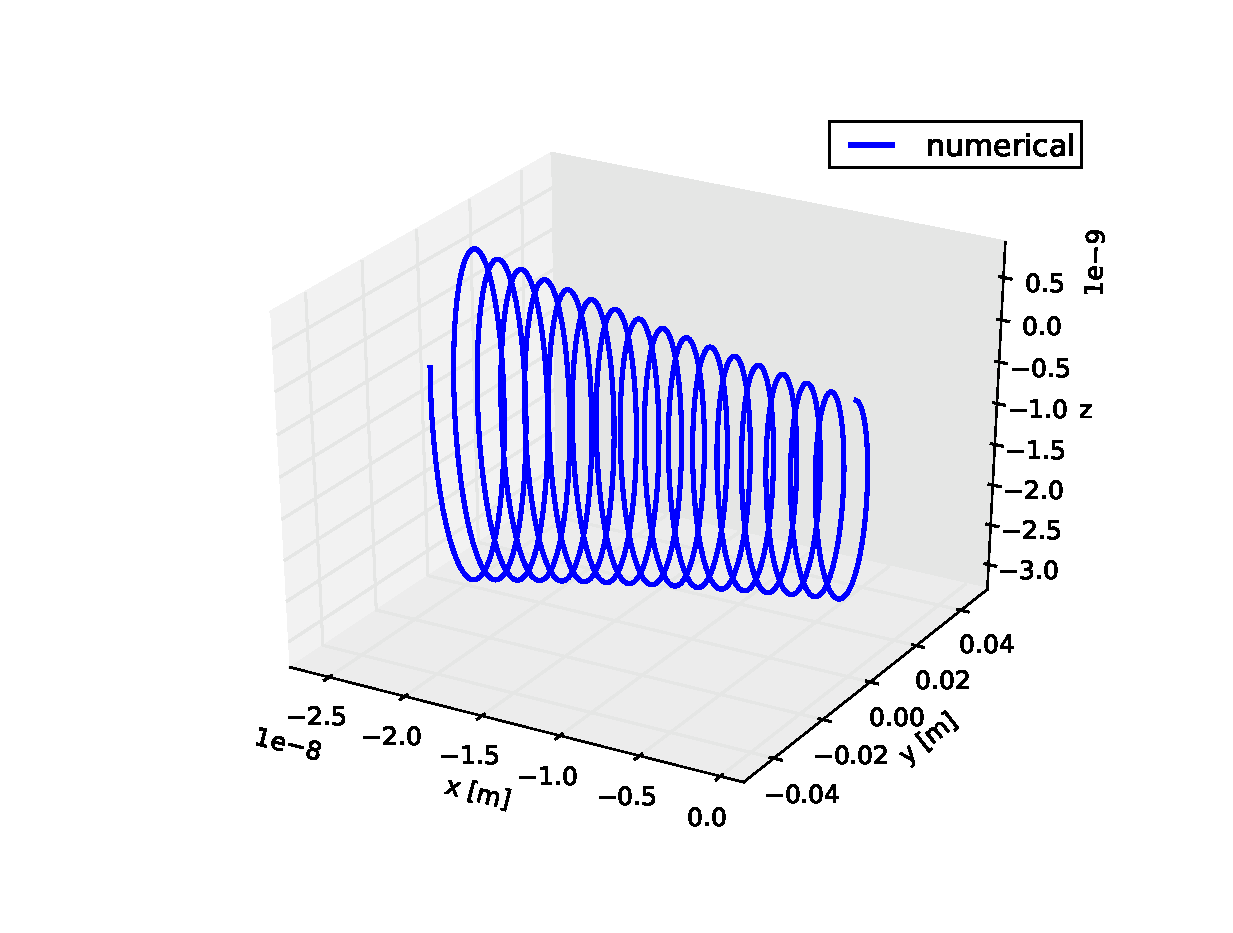
\includegraphics[max size={\textwidth}{\textheight}]{hw6.eps}
\caption{Motion of an electron in an uniform Electric and Magnetic field  }
}
\end{figure}

\noindent The values I computed for the drift velocity is 27.8 m/s, whereas the theoretica value is 25 m/s, which I think is not so far off.

\end{document}